\documentclass[12pt]{article}%[12pt, twocolumn]{aastex631}

\usepackage[a4paper,margin=1in]{geometry}
\usepackage{newtxtext,newtxmath}
\usepackage{graphicx}
\usepackage{float}
\usepackage{amsmath}
\usepackage{natbib}
\usepackage{url}
\usepackage{subcaption}
\captionsetup[subfigure]{skip=10pt}
\usepackage{array}
\usepackage{comment}
\usepackage{tabularx}
\usepackage{booktabs}
\usepackage{afterpage}
\usepackage{xcolor}
\usepackage{listings}

\lstdefinelanguage{SQL}{
    keywords={SELECT, FROM, WHERE, AND, OR, AS, JOIN, LEFT, RIGHT, INNER, OUTER,
              ON, GROUP, BY, ORDER, DESC, ASC, LIMIT, CASE, WHEN, THEN, ELSE,
              END, IS, NOT, NULL, COUNT, AVG, SUM, MIN, MAX, DISTINCT},
    keywordstyle=\color{blue}\bfseries,
    comment=[l]{--},
    commentstyle=\color{gray}\itshape,
    stringstyle=\color{red},
    morestring=[b]',
}

\lstset{
    basicstyle=\ttfamily\small,
    breaklines=true,
    frame=single,
    columns=fullflexible,
    keepspaces=true,
    showstringspaces=false,
    captionpos=b
}

\bibliographystyle{plainnat}

\usepackage[colorlinks=true,
            linkcolor=blue,
            citecolor=blue,
            urlcolor=blue]{hyperref}

\title{\textbf{Exoplanet Transit Classification with Limited Light-Curve Preprocessing Using Convolutional Neural Networks}}

\date{August 27, 2026}
\author{\textbf{Author}: Aaryan Thusoo \\ \textbf{Supervisors}: Prof. Vincent Van Eylen \& (Who is the other?)}

\begin{document}

\maketitle
\pagenumbering{Roman}
\thispagestyle{empty}
\clearpage
\clearpage
\thispagestyle{empty}

\vspace*{\fill}

\begin{center}
\begin{minipage}{0.85\textwidth}

\centering

\vspace{1em}

\raggedright
I want to express my gratitude to my family for their never ending support from back home. Their motivation and belief in me has pushed me to make this paper the best it can be. I could not have pushed through this degree without them by my side.
\\ \vspace{1em}
I would also like to thank Professor Vincent Van Eylen for allowing me to take on this project. The guidance from him along side his PhD student Marina \textbf{(lastname)} and PDRA Kendall Sullivan has been invaluable in coming to the results in this paper. \textbf{(Do I need to provide proper titles for everyone?)}. My appreciation for astrophysics research has only grown with this project and I appreciate their help along the way.

\end{minipage}
\end{center}

\vspace*{\fill}

\clearpage

\newpage
\addcontentsline{toc}{section}{Abstract}
\begin{abstract}
    The use of convolutional neural networks (CNN) to analyse patterns in exoplanet transit signals has been  widely applied for identifying false positive signals. Previous studies commonly focus on substantial preprocessing of the data to improve classification from the model. This paper focuses on improving a CNN model to classify Kepler light curves with limited preprocessing for classification. This included avoiding phase-folding, binning, fitting and other typical tasks used for preparing light curve data. Using lightly processed data, one binary CNN was developed to classify Kepler transiting exoplanets against eclipsing binaries, a common false positive in light curve analysis. A multiclass CNN was also developed to classify light curves from Kepler as transits, shallow or deep eclipsing binaries where a boundary between the eclipsing binary groups was developed for the operations in this work. The binary model evaluation achieved a 92\% accuracy score with 96\% recall indicating the model correctly identified almost all transiting exoplanets. The multiclass model had an accuracy of 78\% and macro averaged F1 score of 79\%. The main source of model confusion comes from the classification difficulty of shallow eclipsing binaries which can mimic exoplanet transit signals. Two random forest models, one binary and one multiclass, were developed as a baseline to compare the performance of the neural networks. The comparison showed the importance of the statistical features of the light curves are as the CNN models achieved similar performance to the random forest models. 
\end{abstract}

\newpage
\tableofcontents
\newpage
\pagenumbering{arabic}
\section{Introduction}

Prior to 1992, the existence of planets beyond the Solar System was largely speculative. This changed with the first observational evidence of extrasolar objects in the early 1990s \citep{First_Exoplanet, First_Exoplanet_RV}. These confirmations transformed the field from theoretical speculation into an observational science. Since then, the rate of discovery has increased rapidly, and by 2008 over 263 exoplanet systems had been confirmed \citep{Exoplanet_numbers_2008}. As of August 2026, over 6000 exoplanets have been confirmed, and thousands more are candidates awaiting further observation \citep{christiansen2025nasaexoplanetarchiveexoplanet}.\footnote{Confirmed planet counts obtained from the NASA Exoplanet Archive Confirmed Planets Table, accessed March 2026: \url{https://exoplanetarchive.ipac.caltech.edu/}}

This rapid growth in detections has been driven by advances in observational techniques and instrumentation. 51 Pegasi b was the first exoplanet discovered orbiting a Sun-like star. It was detected using radial velocity (RV) measurements of its host star \citep{First_Exoplanet_RV}. Although radial velocity measurements remain widely used, transit photometry has become one of the most successful detection methods \citep{How_Many_Transits}. With the development of large-format CCDs, the transit method became the most practical way for large scale exoplanets surveys as wide-field observations allow large numbers of stars to be monitored simultaneously \citep{2005MNRAS.360..703H}.

When analysing transit data, a major source of false positive transit-like signals is eclipsing binary systems, where two stars orbit one another and periodically pass in front of each other from the observer's perspective \citep{2018ApJS..235...38T, Morton_2016}. These systems can produce repeated decreases in observed flux that resemble planetary transits, making them an important contaminant when identifying exoplanet candidates.

This paper trains machine learning models to classify light curves collected from NASA's \textit{Kepler} mission as either transiting exoplanets or eclipsing binaries. Since eclipsing binaries and other astrophysical systems can produce transit-like false positive signals, an automated classifier could reduce the need for manual vetting. Previous studies have explored machine learning approaches for false positive identification, often using heavily processed or phase-folded light curves. The goal of this work is to test whether a model can achieve useful classification performance using relatively limited preprocessing of the input data.


\subsection{Light-Curve Morphology} \label{sec:light-curve-morphology}

Transit photometry observes the flux from stars, searching for periodic decreases in brightness caused by a planet crossing the stellar disk \citep{Exoplanet_Detection_Methods}. This method has become the most successful approach for exoplanet detection, with over 4300 confirmed planets discovered through transits \citep{Num_Transit_Exoplanets_Discovered}. Since transit observations naturally represent stellar brightness as a function of time, a CNN can learn their depth, duration, and shape to make informed estimates of the origin of the data. An example of a Kepler transit light curve is shown in Figure~\ref{fig:example_transit_&_EB}.

\begin{align}
    \delta F \approx \left(\frac{R_p}{R_*}\right)^2 \label{eq:flux_depth}
\end{align}


Astronomers analyse many features in transit light curves which describe key parameters of the exoplanet system. The depth of the transit provides an estimate of the planet-to-star radius ratio, as shown in Equation~\ref{eq:flux_depth} \citep{2010exop.book...55W, 2003ApJ...585.1038S}. Here $\delta F$ is the change in normalized flux caused by the transit dip, while $R_p$ and $R_*$ represent the radii of the exoplanet and host star, respectively. As the ratio of radii between a planet and star is relatively small, planetary transits usually produce shallow decreases in flux. In eclipsing binary systems, the occulting body is another star, so the radius ratio is generally larger and the resulting eclipse depth is often but not always greater than that of a planetary transit.

\begin{figure}[h]
    \centering
    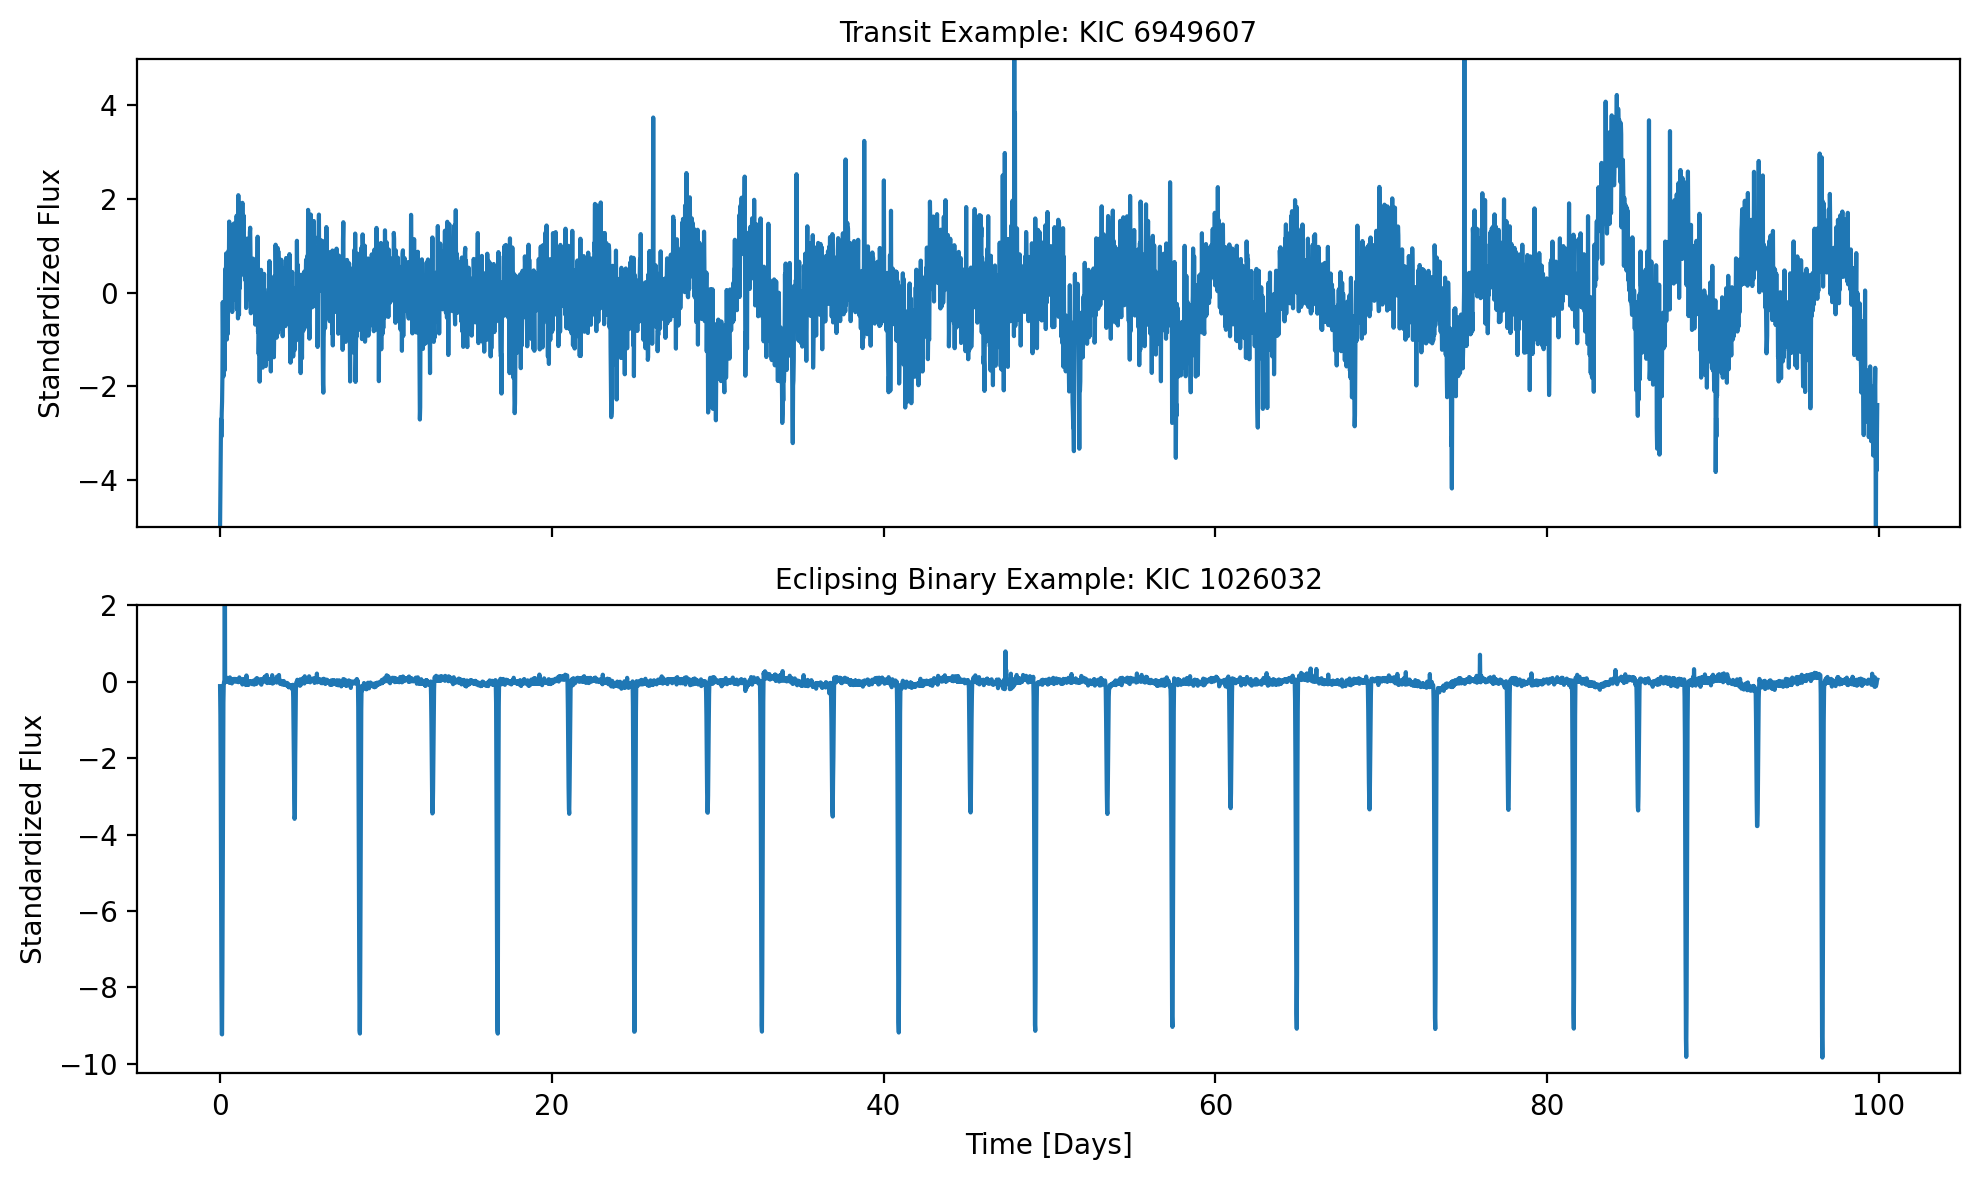
\includegraphics[width=0.99\linewidth]{figures/images/lightcurve_examples.png}
    \caption{Examples of the one-dimensional Kepler light curves used in the model training done in this paper. The plots show a 100-day chunk of KIC 6949607 and 1026032, the light curves of stars hosting a confirmed transiting exoplanet and confirmed eclipsing binary respectively. The model looks for features such as the dips and their duration and shape to classify the data as a transiting light curve. It can be seen how the transit example shows repetitive dips of relatively same depth while the eclipsing binary has a clear different in the two eclipses. The eclipsing-binary instance shows more pronounced dips in the standardized light curve, with the eclipse events extending further below the standardized baseline.}
    \label{fig:example_transit_&_EB}
\end{figure}

Transit shape also contains useful information. The ingress and egress are the times when the planet begins and ends its passage across the stellar disk, while the duration represents the total time spent between ingress and egress \citep{2010exop.book...55W}. Transiting exoplanets usually produce rounded, U-shaped dips, whereas eclipsing binaries can produce sharper V-shaped features that may resemble planetary-like signals \citep{2010exop.book...55W}. It is important to note that transits may also produce sharper V-like dips in the case of a grazing transit, where the planet does not fully pass across the stellar disk. Similarly, eclipsing binaries can produce more U-shaped eclipses depending on the geometry of the system \citep{2017MNRAS.465.2634A}. Thus, the shape is a useful tool for classification but is better combined with other factors for final predictions.
\input{sections/detection_challenges}
\input{sections/missions}
\input{sections/pipelines}
\input{sections/methods}
\input{sections/results}
\section{Discussion}

The goal of this paper is to accurately classify light curves as representing potential exoplanets amongst many false positive cases. The binary model focused on the most common false positive occurring from eclipsing binary systems. The multiclass model attempts to include a separation between deep eclipsing binaries and shallow eclipsing binaries. Further cases can be added to give more possible classifications but for now the most important categories were covered.

The results found in this work demonstrate that 1D CNNs can distinguish confirmed transiting systems from eclipsing binaries with high performance. Unlike other papers, these results come from minimally processed Kepler light curves and show time can be saved on processing the data. However, there was still some classification difficulty as the eclipsing binary population produced non uniform errors, with shallow depth eclipsing binaries representing the principal source of confusion. 

\textbf{(Should I add a comparison to other papers which used higher preprocessing?)}

The data preparation did not apply any sigma-clipping of the normalized light curves. This was due to previous experiments showing that any application of clipping reduced the binary model across all metrics. The final decision to remove clipping, was motivated by the concern of outlier rejection accidentally removing important astrophysical information. Table~\ref{tab:clipping_comparison} shows the difference in the binary model metrics when applying sigma clipping to when it was not used.

\begin{table}[h]
    \centering
    \begin{tabular}{lccc}
        \hline
        \textbf{Metric} & \textbf{Sigma Clipping} & \textbf{No Clipping} & \textbf{Improvement} \\
        \hline
        Accuracy  & 83.28\% & 93.17\% & +9.89 pp \\
        Precision & 79.18\% & 89.46\% & +10.28 pp \\
        Recall    & 91.64\% & 98.50\% & +6.87 pp \\
        F1 Score  & 84.95\% & 93.76\% & +8.81 pp \\
        ROC-AUC   & 0.881   & 0.978   & +0.097 \\
        \hline
    \end{tabular}
    \caption{Comparison of binary CNN performance with and without sigma clipping during light-curve preprocessing. The improvement represents the absolute percentage-point change after removing sigma clipping, with ROC-AUC reported as an absolute change. Due to the improvements, sigma clipping was therefore excluded from all models.}
    \label{tab:clipping_comparison}
\end{table}

The binary model produced strong results which indicate it is very efficient in classifying distinctions between real and fake transit cases. Table~\ref{tab:metrics_table} shows the favourable results from the binary model test. An accuracy of 93\% indicates the model does not overall struggle handling the data. The precision and recall of 88\% and 98\% respectively show there is little to no issue classifying true transits appropriately. The recall shows the model found almost all of the transits which were used in the test. The precision however represents the reliability that a transit classification is truly a transit. While it is high, there is still 12\% of transit classifications which were actually eclipsing binaries.

While some light curve instances contained unusual features which may affect classification, there are also cases which manage to trick the binary classifier. Figure~\ref{fig:good_vs_bad_examples} shows a collection of correctly and incorrectly classified example instances used in testing. For the correctly classified cases, the top left plot shows a true transit instance. It appears visually similar to the top right plot, which depicts a false positive eclipsing binary. This demonstrates the difficulty of working with the intricate light curve data, as visually similar standardized inputs can result from different classes.

As for the eclipsing binaries, the bottom left shows an instance which was correctly classified. The alternating eclipse depths provide a clear feature expected from an eclipsing-binary system. The bottom right plot is a transit incorrectly classified as an eclipsing binary. Repeated downward features with varying standardized depths can be observed in the data, which may have contributed to the model incorrectly identifying the instance as an eclipsing binary. The exact source of these features cannot be determined from the light curve alone and could result from astrophysical variability, instrumental effects, or the processing of the observations.

\begin{figure}
    \centering
    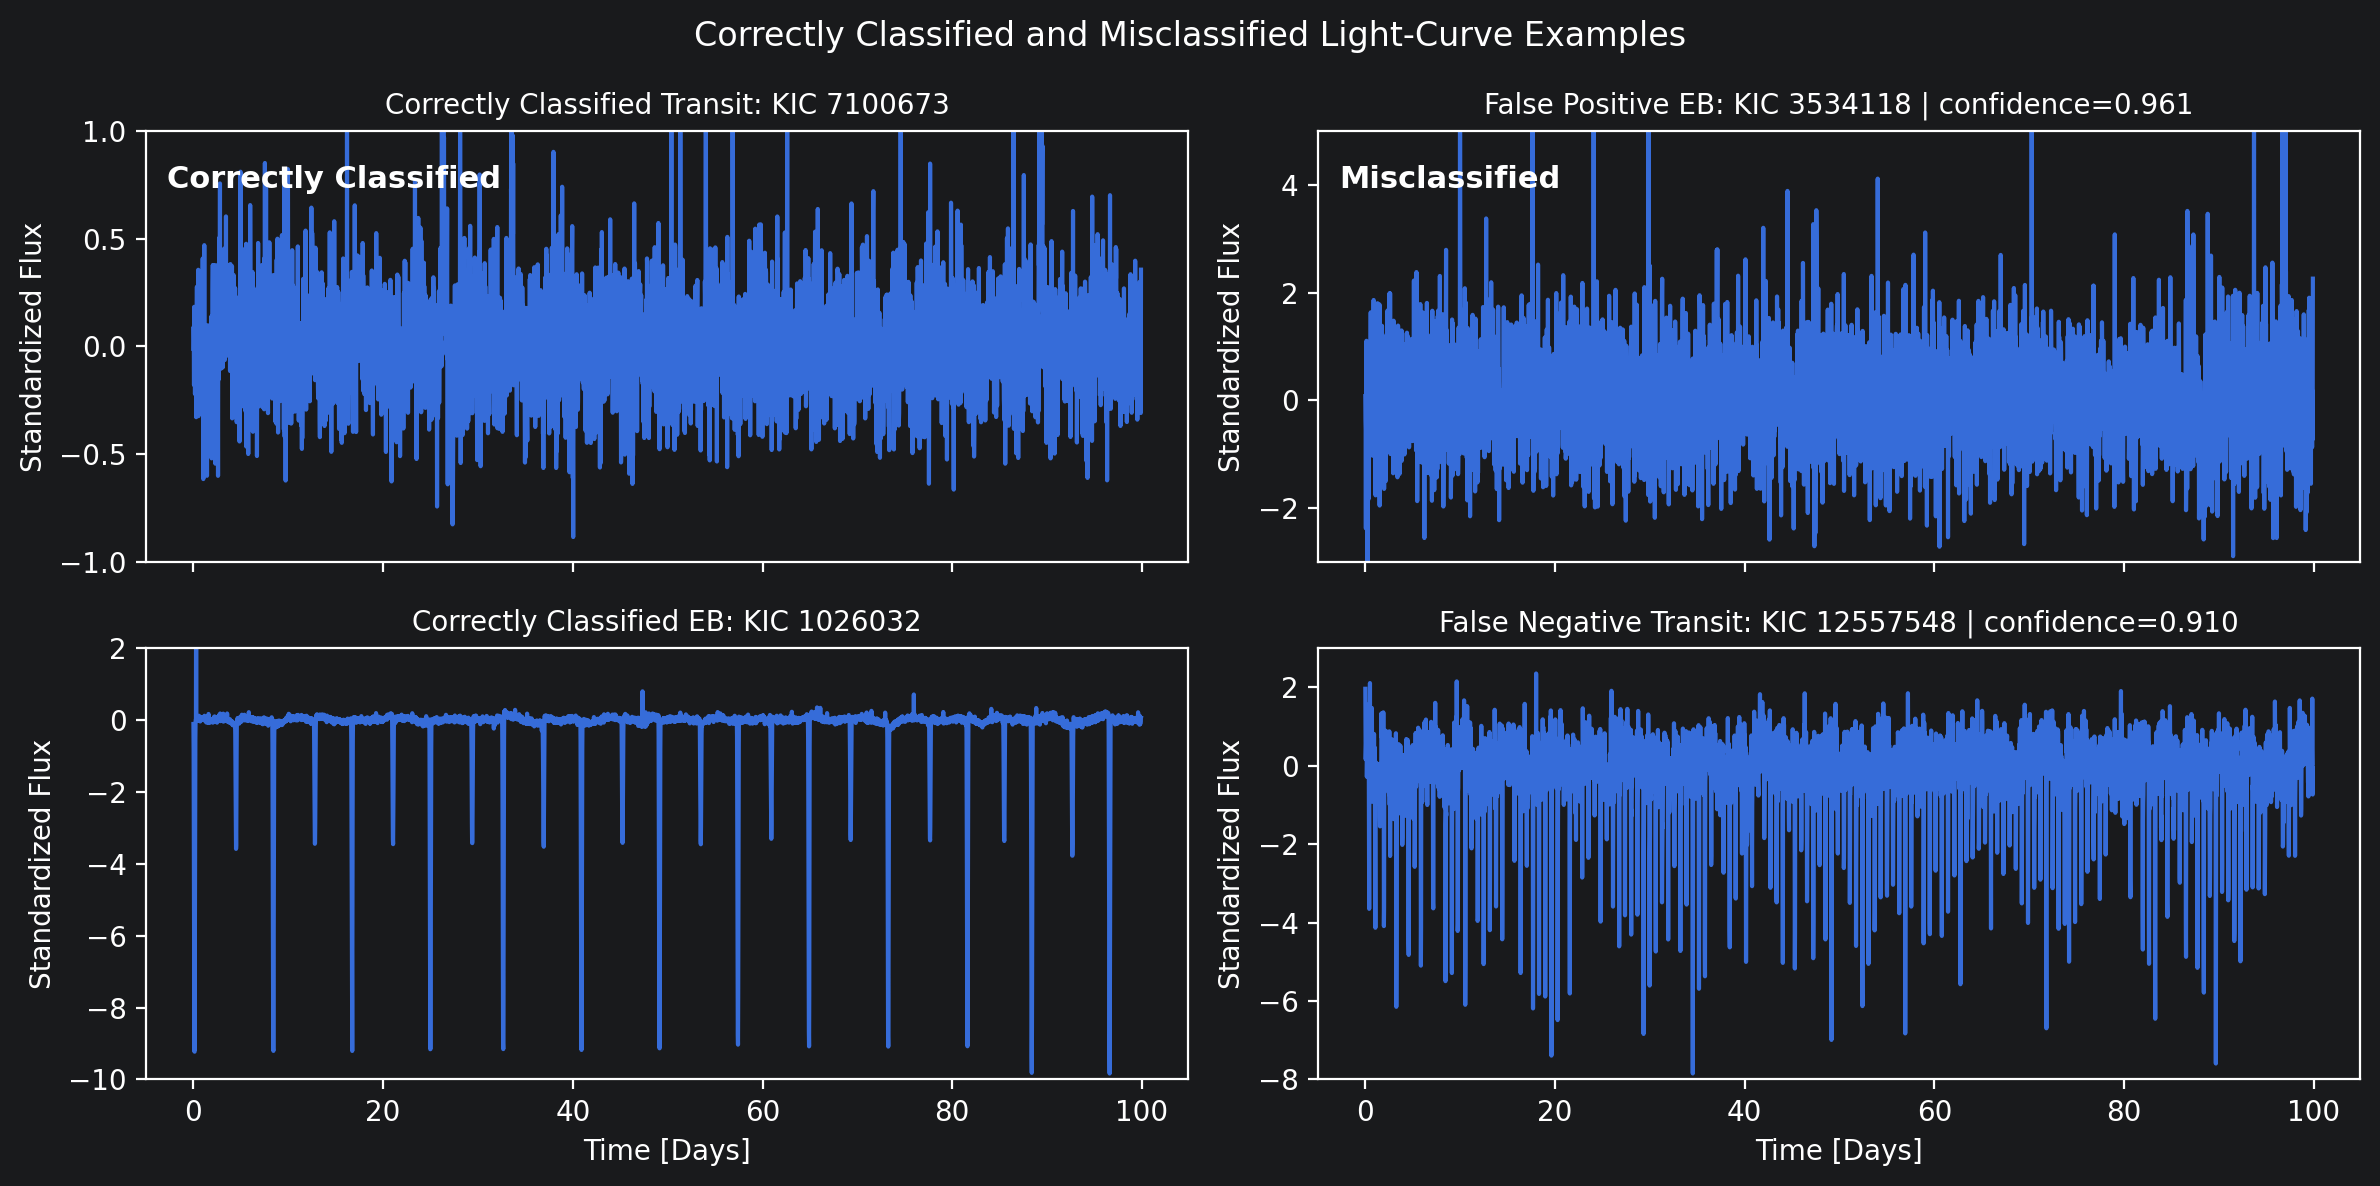
\includegraphics[width=0.9\linewidth]{figures/images/good_bad_binary_examples_2x2.png}
    \caption{Examples of correctly classified and misclassified light curves from the binary CNN. The left column shows correctly classified instances of a transit and eclipsing binary 100-day chunk. The right column shows an instance of both a transit and eclipsing binary which was misclassified by the binary model. The light curves shown are from after standardization and represents exactly the data provided to the model for training and testing. Limits on the plotted y-axis were applied to focus on the main density of data exclusing outliers.}
    \label{fig:good_vs_bad_examples}
\end{figure}

It can be seen from the confidence histogram that a large number of misclassified instances were found in the high-confidence ranges. One likely factor is the depth of the transits or eclipses, which can first be seen in the box plot in Figure~\ref{fig:depth_boxplot_fp}, where the high-confidence group has the most consistent collection of low-depth cases. This is further supported by the high-confidence false positives, where over 80\% of the unique systems were matched to shallow eclipsing binaries. This suggests that the shallow EB class is important to separate from the transit and deep EB cases, as these systems can be confidently mistaken for exoplanet-like transits.

The final decision for a split between shallow and deep eclipsing binary cases was needed for creating the multiclass model and Figure~\ref{fig:mc_threshold_find} gave the best representation for determining the threshold. The histogram shows how majority of misclassified eclipsing binaries come from relative eclipse depths of 0.01 or less. Totalling up the ratios, 42.1\% (160/380) of eclipsing binaries with depths less than 0.01 were misclassified while only $\sim1.0\%$ (11/1073) of those with depths greater than 0.01 being misclassified. The substantial difference in confusion rate provides good justification for the 0.01 operational depth split boundary.

Compared to the binary CNN model, the multiclass model performed a little poorly across the evaluation metrics. However this result is expected as this model deliberately introduces the difficult shallow eclipsing binary class. The accuracy while lower still shows the model is successful about 79\% of the time. The precision and recall are both similar in value at 80\% and 78\% respectively which indicates the model does not favour a certain class.  

Looking at the confusion matrix, the multiclass model was successful in classifying transits and deep eclipsing binaries. There were only 5 deep eclipsing binaries wrongfully classified as transits while no transits were classified as deep eclipsing binaries. The main difficulty was the shallow eclipsing-binary class, which contains features similar to both edge cases. The majority of errors involved the shallow eclipsing-binary class, with 25.9\% of shallow cases being classified as transits. As well, 15.6\% of deep eclipsing cases were classified as shallow. Overall, 140 of the 145 misclassifications either came from or were classified into the shallow eclipsing-binary class. This was expected and was the overall reason for creating the multiclass model. Figure~\ref{fig:mc_threshold_find} showed most binary-model misclassifications were associated with the shallower eclipse depths, and so having the majority of errors in the multiclass case involving the shallow eclipsing-binary class further supports the relationship between eclipse depth and classification difficulty. Therefore, while the metrics show poorer performance, the main source of difficulty is separated into its own class.

The shallow eclipsing binaries have depths similar to transits but also feature patterns expected of eclipsing binaries. Physically, these shallow eclipses can be caused by a few different cases. One occurrence is dilution from a third stellar light source being picked up in the observations, which can reduce the observed eclipse depth \textbf{(citation)}. As well, if the eclipse is grazing and only a small portion of the opposite star is obscured, the resulting dips can be less pronounced \textbf{(citation)}. Shallow eclipsing binaries therefore represent an important source of ambiguity when distinguishing eclipsing binaries from transiting systems. The multiclass results support making this distinction, as separating the shallow eclipsing binaries into their own class isolated the majority of classification errors from the more clearly separated transit and deep eclipsing-binary cases.

The random forest model produced results which were similar to the CNN model. This is important because the random forest does not learn directly from the full shape of the light curve in the same way as the CNN. Instead, it uses extracted features such as the mean flux, standard deviation, minimum flux, maximum flux, and chunk depth. The similar performance suggests that these simple statistical features already contain a large amount of information needed to separate transits from eclipsing binaries. Therefore, while the CNN is useful because it can learn directly from the light-curve shape, the random forest results show that the simple summary statistics may be highly informative for classification problems.

\subsection{Limitations}



\subsection{Potential Future Actions}

Overall this paper focused on transits and eclipsing binaries. By splitting into shallow and deep eclipsing binaries the near eclipsing binary case is also covered. However there are several other potential false positive cases to look into. \textbf{(Figure out what they are and cite them. Ask Marina)}. For a model useful for new data, other cases must be taken into account. 

A major focus of this paper was the use of limited preprocessing to test how well the models could perform without heavily preparing the light-curve data. In the pipeline used for this research, the main processing step was the application of the Savitzky-Golay filter from the \texttt{lightkurve} package. No binning, phase folding, or heavier filtering was applied, reducing the amount of preprocessing required before classification. Based on the results of this paper, introducing some additional processing into the pipeline may improve model performance. However, the balance between preprocessing time and classification performance would need to be tested to determine the best approach. This may be especially important for shallow or noisy signals, where the model struggled most.

As stated in the methodology, the data preparation steps include a second standardization step outside of the \texttt{lightkurve} package. The model must have a baseline for the data to work from as well as a more controlled numerical scale between the light curves. The current standardization median-centres each light curve and divides it by its standard deviation. This means the original relative eclipse depth is not directly preserved, as the depth is instead scaled relative to the variability of each light curve. The way the standardization is done, however, can be changed to potentially produce more favourable results. \textbf{(Cite those papers which Marina showed removed depth as a factor)} showed the model can be run with the data scaled between 1 and -1. This further reduces the importance of the original depth by making all instances stretch across the same range. Using this normalization strategy could improve the model by making it focus more on the morphology and shape of the light curves. Since transits and eclipsing binaries typically generate differently shaped dips, this could improve the performance of a pattern recognition model such as a convolutional neural network.

CNN models can also be injected with extra information. \textbf{(Also get those papers about injecting things like radius ratio and impact parameter)} shows the application of physical parameters such as flux ratio and impact parameter. They use several convolution layers, different set up to the architecture used here, but before proceeding to the dense layer, feature values are provided to the network. The random forest results in this paper have shown the importance of features over the entire data set. While this paper is focused on using minimal data processing, finding a balance with feature injection can improve future models. 

There are a few things which could be done in a future project to improve results. The model layers can be altered to include more convolutions or dense learning layers. More convolution would help to create larger feature maps for the model to compare from. As well altering kernel sizes to fit more data in the filter could be helpful. The use of dropout to limit overfitting appears to have worked correctly and thus adding more overfitting prevention steps likely will not improve results. As the data is relatively simple for the CNN, massively increasing the number of layers is unlikely to provide noticeable improvements. The model used TensorFlow Keras layers which work very well but the library also allows for custom layers to be developed. Utilizing this, it may be possible to make a convolution layer customized for the specific case of light curve classification. 

Models can also be trained using other models and this method is utilized in many machine learning cases across different fields. One way to use this in this work could be to develop synthetic data to initially train the model off of. If the generated data is made to be statistically significant compared to the real Kepler data, it can be used to make a basic starting model. Then, by creating a strong model off the synthetic light curves, the architecture can be reused on real data to potentially struggle less with the classification of real light curves.  

\begin{comment}
Is any of this useful to mention here?

\subsection{Transiting Exoplanet Survey Satellite (TESS)} \label{sec:TESS}

\begin{figure}[h]
    \centering
    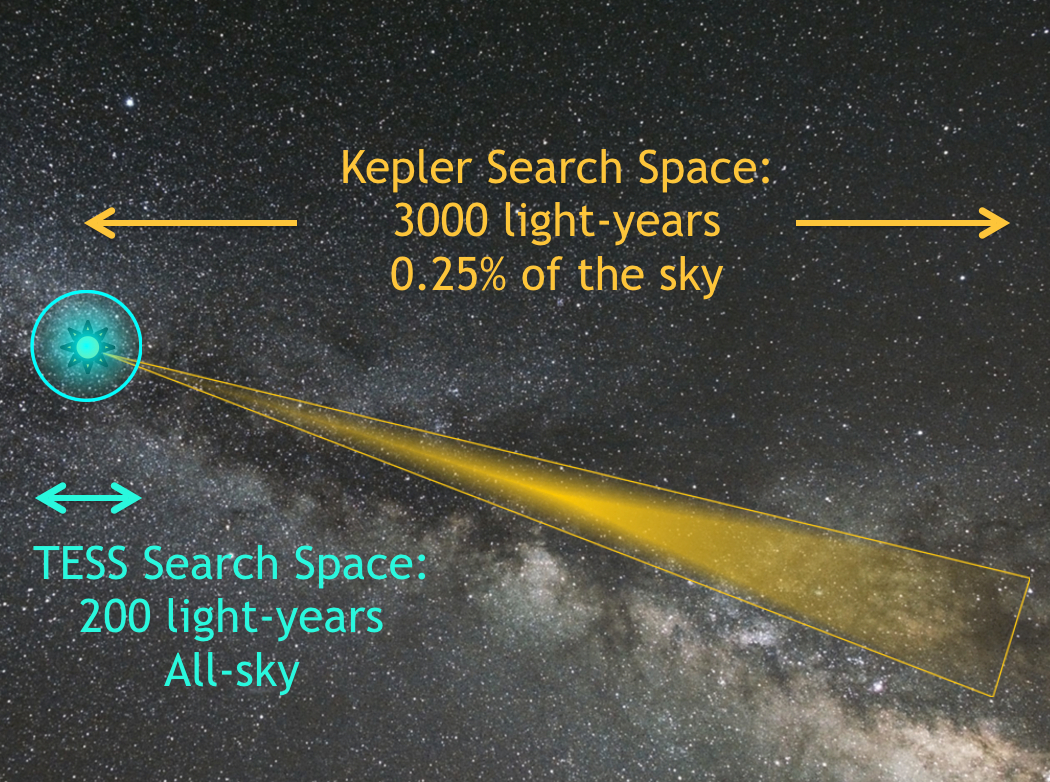
\includegraphics[width=0.9\linewidth]{figures/images/TESS_vs_Kepler}
    \caption{Comparison of the survey strategies of the \textit{Kepler} and TESS missions\protect\footnotemark[4]{}. \textit{Kepler} focused on a deep search of a small region of the sky, while TESS conducts a wide-field survey targeting nearby stars across nearly the entire sky.}
    \label{fig:TESS_vs_Kepler}
\end{figure}

\footnotetext[4]{\url{https://www.nasa.gov/space-science-and-astrobiology-at-ames/division-overview/astrophysics-branch-overview-sta/exoplanet-mission/exoplanet-research-projects}}

Following the success of the \textit{Kepler} and K2 missions, NASA launched the Transiting Exoplanet Survey Satellite (TESS) to carry out a wide-field survey of nearly the entire sky, focusing on nearby, bright stars well suited for follow-up characterization \citep{Ricker2015, Huang2018}. This observing strategy puts emphasis on short-period planets orbiting luminous host stars which are better suited for precision mass measurements and atmospheric studies.

TESS monitors the sky in sectors with typical observing baselines of $\sim27$ days each. Compared to \textit{Kepler}, which maintained continuous observations of the same field, this is significantly shorter. Figure~\ref{fig:TESS_vs_Kepler} shows an artist rendition of the field of view covered by TESS in comparison to that of \textit{Kepler}. As a result, TESS is most sensitive to planets with orbital periods shorter than $\sim10$–$20$ days. Longer period planets remain better constrained by the extended \textit{Kepler} dataset \citep{Sullivan2015}. Despite this limitation, TESS has greatly expanded the known population of transiting exoplanets and produced thousands of candidates orbiting bright nearby stars across the sky \citep{Guerrero2021}.

Together, \textit{Kepler} and TESS complement one another on insights into exoplanet populations. The long baseline and high photometric precision of \textit{Kepler} allowed for statistical studies of population occurrence rates and structure. One prominent result is the discovery of the “radius valley”, a deficit of planets with radii around $1.5$–$2R_{\oplus}$ that separates two dominant populations of super-Earths and sub-Neptunes \citep{2017AJ....154..109F, 2018MNRAS.479.4786V}. In contrast, TESS primarily detects planets orbiting bright nearby stars, making these systems well suited for detailed follow-up observations. These include radial velocity mass measurements and atmospheric characterization with facilities such as the James Webb Space Telescope. TESS is the connection between the statistical studies of exoplanet populations and parameter estimation of planetary systems \citep{Batalha2019}.

\subsection{PLAnetary Transits and Oscillations of stars (PLATO)} \label{sec:PLATO}

Looking ahead, the European Space Agency (ESA) is preparing the next major mission in exoplanet transit research. Known as the \textit{PLAnetary Transits and Oscillations of stars} (PLATO) mission, its objective is to extend the work \textit{Kepler} and TESS by introducing high-precision, long-baseline photometric monitoring of bright stars across large areas of the sky \citep{Rauer2014}. The mission is currently scheduled to launch between late 2026 and early 2027. PLATO's primary goal is to detect and characterize terrestrial exoplanets orbiting within the habitable zones of their host stars. Furthermore, the mission will perform asteroseisomology to determine precise stellar ages, radii, and masses.

PLATO will combine wide-field coverage with long-duration observations lasting several years in selected fields. In contrast to TESS, PLATO's strategy is optimized for detecting small planets with longer orbital periods which are much more difficult to observe with current all-sky transit surveys \citep{Rauer2014}. The mission is expected to produce a statistically robust sample of Earth-sized planets with well constrained host-star properties. Such measurements will enable detailed study of planetary system evolution and improve estimates of habitable worlds in the solar neighbourhood. 

Together, PLATO, \textit{Kepler}, and TESS form a complementary sequence of transit surveys. Collectively, they span deep narrow-field observations, all-sky coverage of bright stars, and future baseline characterization of nearby terrestrial systems.  Within this progression, PLATO is anticipated to provide the precise stellar and planetary parameters necessary to connect statistical exoplanet demographics with detailed physical characterization \citep{PLATO2022}.
\end{comment}
\section{Conclusion} \label{sec:Further_Steps}

This work aimed to develop a convolutional neural network that can classify exoplanet transit light curves while applying limited processing to the data. Other papers have applied heavy preprocessing as well as strong neural networks to achieve positive results. This paper showed an introduction to using simpler models with less provided information while maintaining results which are optimistic for future work.

First a binary model was developed which simply classified light curves between true exoplanet transits and eclipsing binaries. With the results from this model evaluation, the depth appeared to be a very important feature for the binary models classification and thus a more difficult 3-class CNN was developed. This model aimed to split the eclipsing binary dataset into shallow and deep groups based on the depth from the the normalized flux. 

The binary model returned a 92\% accuracy score indicating the majority of test data was correctly classified while the 88\% precision score warns that the model did classify a non-negligible batch of eclipsing binaries as transits. For a usable model this precision score is the most important to look into further. 

The multiclass model did not perform as well as the binary but the results did show the depth of transits was the major feature affecting the models decisions. As the results are macro-averaged, it is understood the shallow eclipsing binary class was the most challenging for the model. The CNN would mix up both transits and deep eclipsing binaries as the shallow case and this lowered all final metrics to the high 70s.

The main takeaway from this paper is the impact of depth for the classification problem. The results of both CNN models, between their confusion matrices and analysis of the misclassified instances, show the depth is correlated to the ability of the models to classify light curves correctly. 

The introduction of random forest models proved the CNN models are building off of the baseline. Both classifiers use different processes, with the random forest using inputted values while the CNN observes the light curve as a whole. It is clear the simple values such as depth, and flux ranges are important for classification. Potentially a future pipeline could combine calculated values and the CNN to make a more efficient combined model. 

This paper faced a few limitations which had to be followed. The first is the number of available confirmed exoplanet transits and valid eclipsing binaries. These were the only labelled Kepler objects that could be reliably used and in the future having more data to train and test off of will help later models. Without increasing the architecture of the CNN model, the classification was limited to 3 classes while there are several other potential false positive situations. 

The approaches in this paper work reasonably well for managing lightly processed Kepler data. As Kepler is a well documented mission, this makes for a great starting point for developing useful classification models. Shallow depth eclipsing binaries are the main obstacle for future models to handle.

\newpage


\bibliographystyle{plain}
\bibliography{references}

\newpage 
\appendix \label{sec:Appendix}

\section{Neural Network Metric Equations} \label{sec:NN_equations}

The first metric is the accuracy which is simply the number of correct results divided by the total number of test instances. An accuracy of X\% indicates the model returns the correct classification X\% of the time. This is good as a base but does not give information about the models classification of certain classes.

The following metrics are based on positive and negative results where positives are the wanted result while negatives are for the unwanted result. For this papers binary model, a positive result was a transit classification while eclipsing binaries were negative results. Each metric and their equation used in this work is shown below. T and F stand for True and False while P and N stand for Positive and Negative. R means Rate so for example FPR means False Positive Rate.

\begin{align}
    \text{Precision} = \frac{TP}{TP+FP} \label{eq:precision}
\end{align}

The precision equation is shown above in Equation~\ref{eq:precision}. This metric asks, of all the positive results returned by the model, what fraction of them were truly positive results. Precision in this paper tells how many transits are being missed and is important for understanding if the model will lose a large amount of important results. Below in Equation~\ref{eq:recall} is the recall equation. This metric asks, of all the actual positive results, how many did the model find. For the context of this work, the recall indicates how many transits are found by the model.

\begin{equation}
    \text{Recall} = \frac{TP}{TP+FN} \label{eq:recall}
\end{equation}

\begin{equation}
    F_1 = \frac{2TP}{2TP + FP + FN}
\end{equation}

\begin{align}
    AUC &= \int_0^1{\text{Recall}(FPR)d(FPR)}, \textbf{ where} \\
    FPR &= \frac{FP}{FP + TN}
\end{align}


\section{KOI SNR Analysis}

The same analysis was repeated using the signal-to-noise ratio saved in the Kepler archive. The values are not on the same scale as the calculated SNR so the distributional pattern is the more important feature to observe. Below, Figure~\ref{fig:koi_snr_boxplot} shows the box plots for the archive SNR split again into confidence groups. Similar to the calculated SNR, the false positive cases with low to medium confidence display a wide range of archive SNR values. There are also few high confidence false positive values so no clear conclusion can be made. In the false negative case, all three confidence groups again do not show a clear separation by confidence groups.

\begin{figure}[htbp]
    \centering

    \begin{subfigure}[b]{0.48\textwidth}
        \centering
        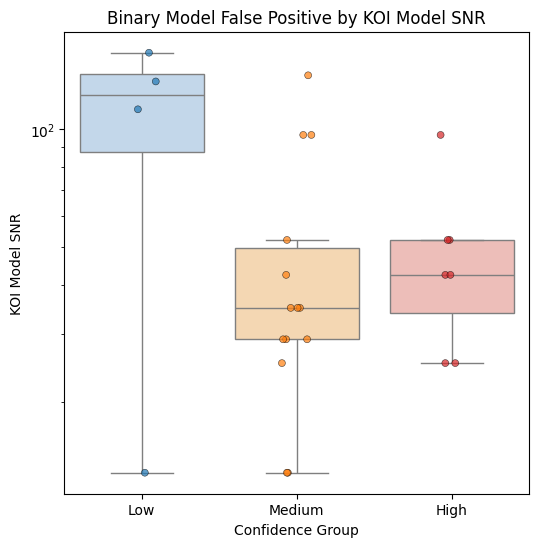
\includegraphics[width=\textwidth]{figures/plots/fp_boxplot_koi_model_snr.png}
        \caption{Boxplot of Kepler SNR values for false positives}
        \label{fig:koi_snr_boxplot_fp}
    \end{subfigure}
    \hfill
    \begin{subfigure}[b]{0.48\textwidth}
        \centering
        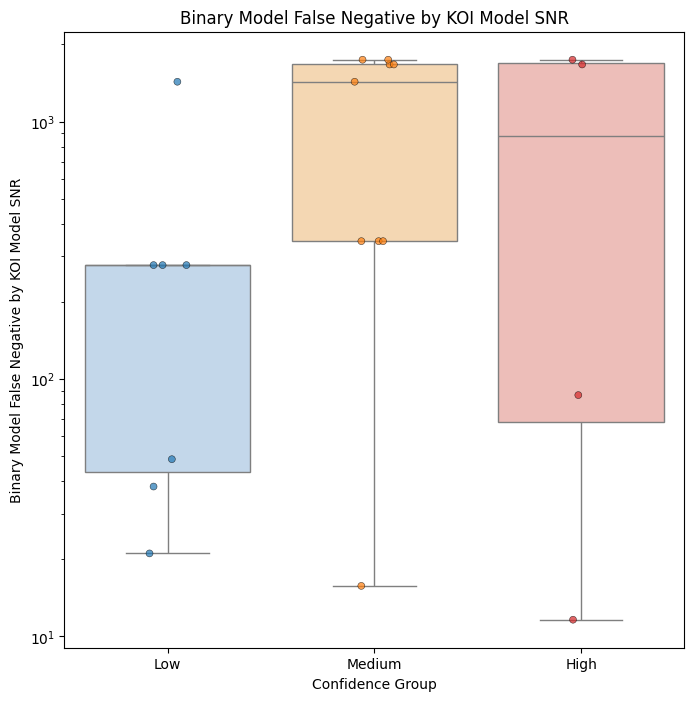
\includegraphics[width=\textwidth]{figures/plots/fn_boxplot_koi_model_snr.png}
        \caption{Boxplot of Kepler SNR values for false negatives}
        \label{fig:koi_snr_boxplot_fn}
    \end{subfigure}

    \caption{Boxplots of the Kepler archive SNR values of misclassified test light curves. They are split by low, medium, and high confidence values.}
    \label{fig:koi_snr_boxplot}
\end{figure}

Another expression of the signal to noise results is shown in Figure~\ref{fig:snr_ratio_bottom}. These plots show the incorrect classification ratio for low, medium, and high SNR groups again split by low, medium, and high model confidence. Here, the correct results are also incorporated and now the full test set context is used. The mistake count for each bin is divided by the total number of samples in each SNR/confidence bin.

\begin{figure}[h]
    \centering
    \begin{subfigure}[b]{0.48\textwidth}
        \centering
        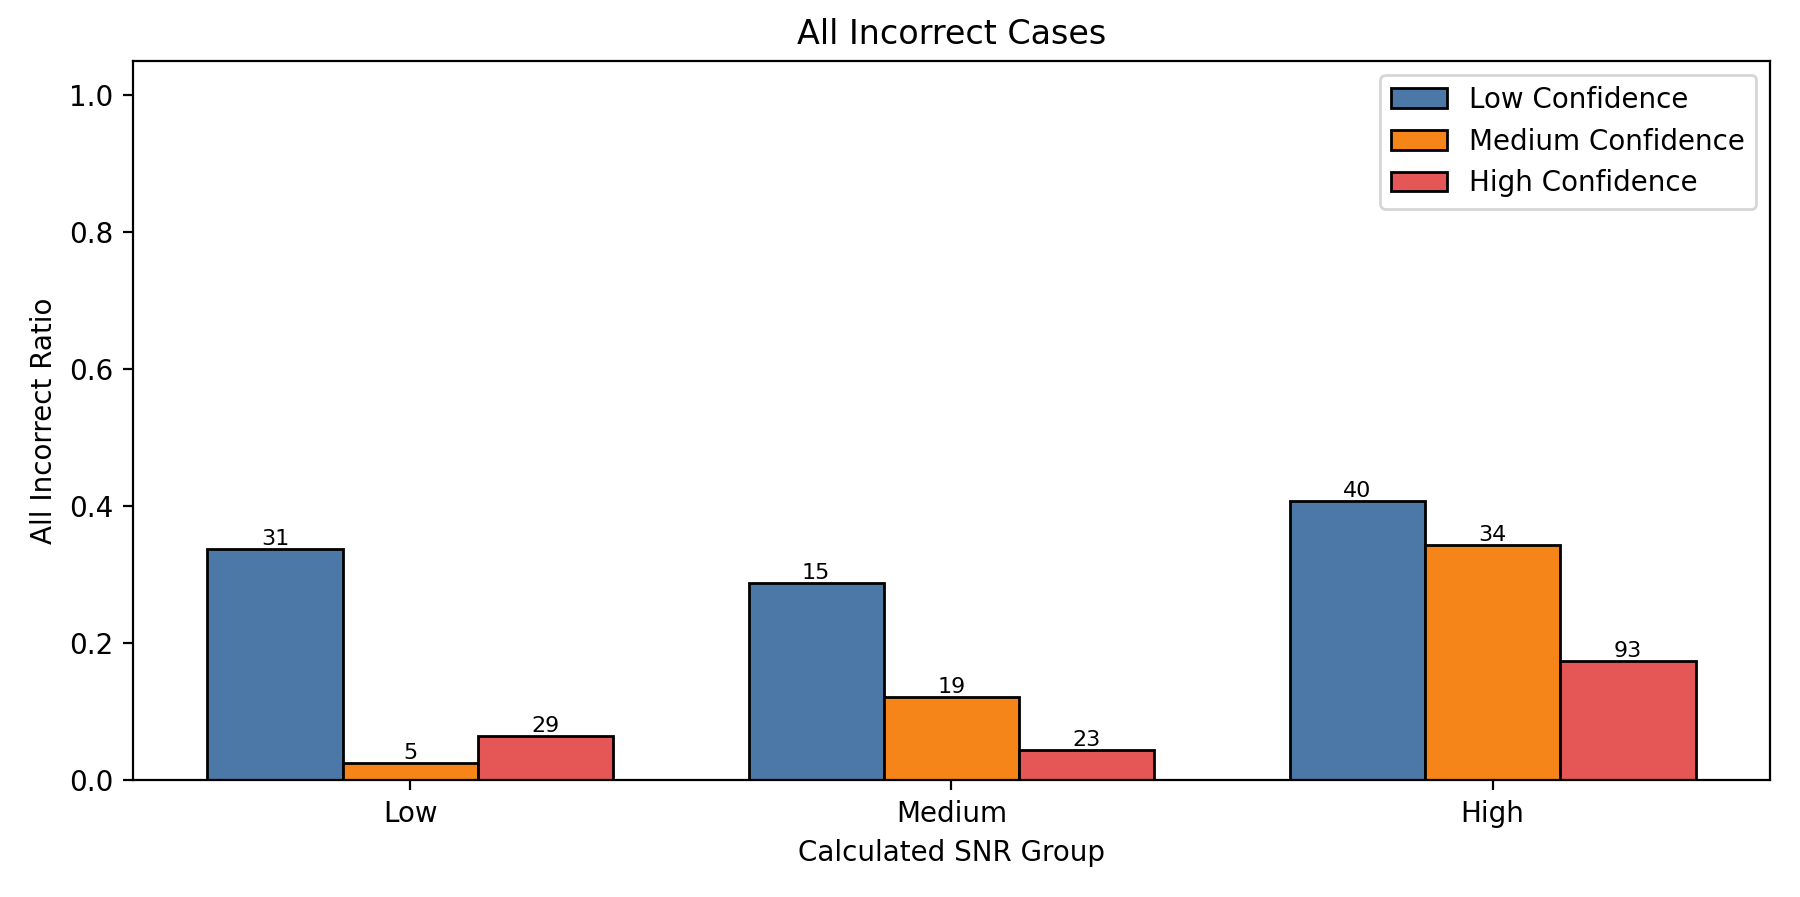
\includegraphics[width=\textwidth]{figures/plots/mistake_ratios_by_calculated_snr_and_confidence_bottom.png}
        \caption{Calculated SNR}
        \label{fig:calc_snr_ratio_bottom}
    \end{subfigure}
    \hfill
    \begin{subfigure}[b]{0.48\textwidth}
        \centering
        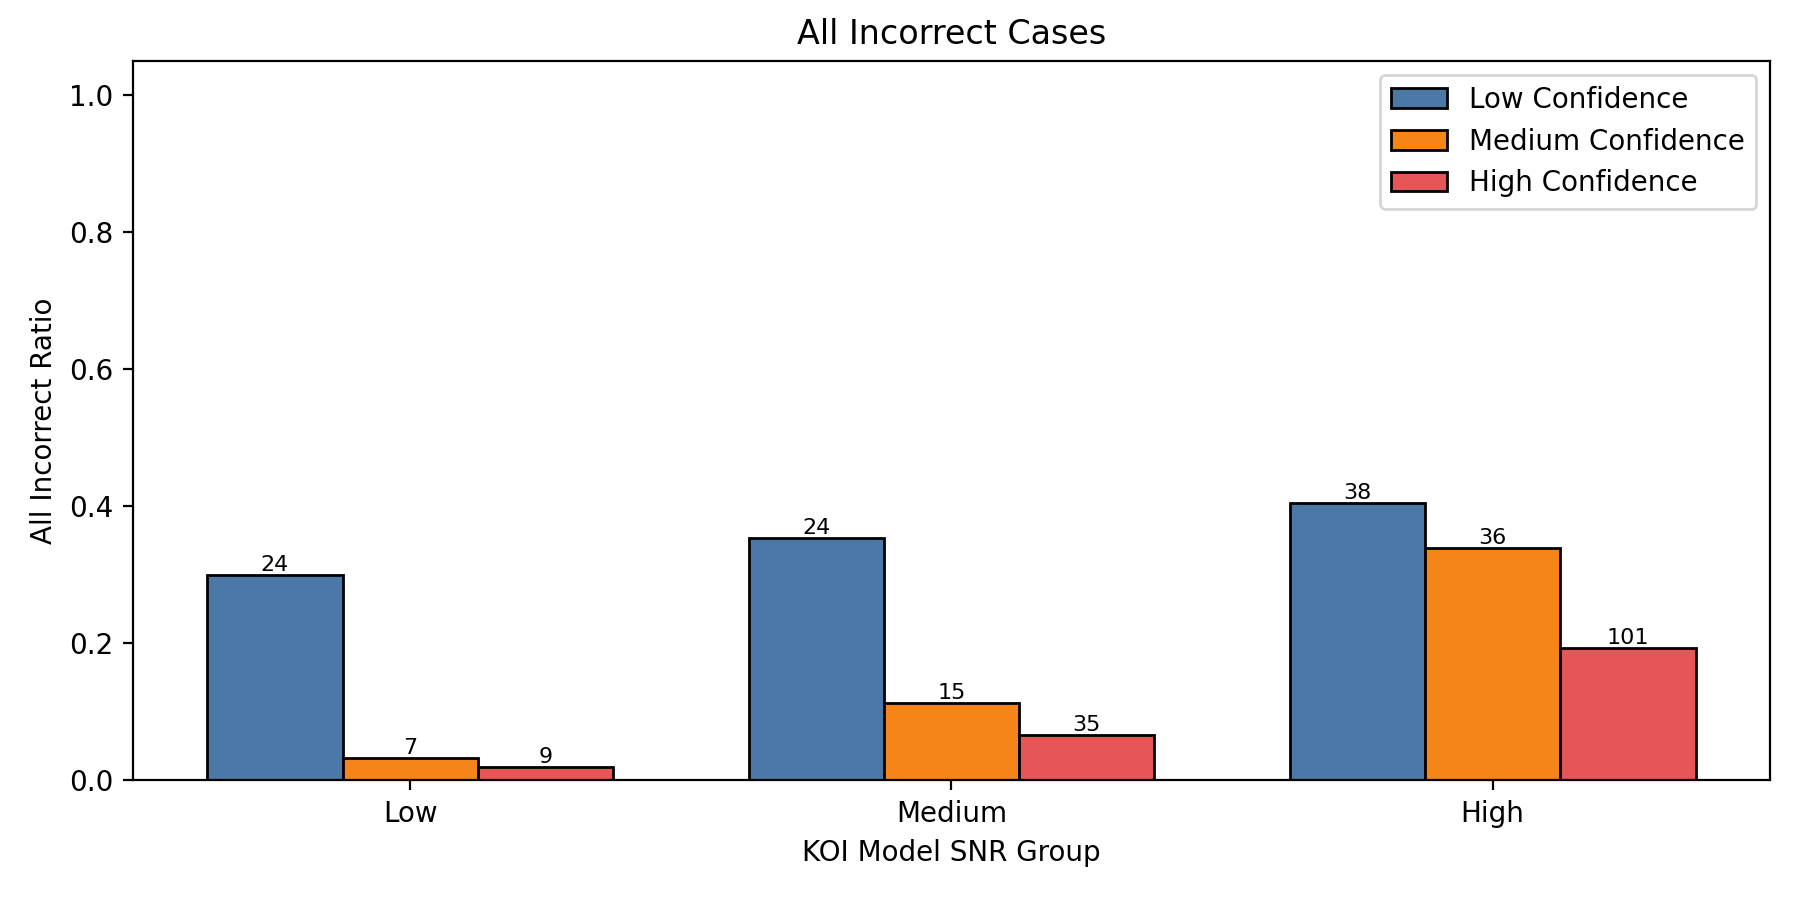
\includegraphics[width=\textwidth]{figures/plots/mistake_ratios_by_koi_model_snr_and_confidence_bottom.png}
        \caption{KOI model SNR}
        \label{fig:koi_snr_ratio_bottom}
    \end{subfigure}

    \caption{Incorrect classification ratio across SNR groups and confidence groups.}
    \label{fig:snr_ratio_bottom}
\end{figure}

\begin{comment}
\section{Transit Geometry} \label{sec:Transit_Geometry}

Several parameters describing the geometry of a transiting exoplanet system can be derived from the transit light curve. One of the most important is the impact parameter $(b)$, defined as the projected distance between the centre of the stellar disk and the transit chord:

\begin{align}
    b = \frac{a\cos{i}}{R_*}
\end{align}

Here, $a$ is the semi-major axis of the orbit, $i$ is the inclination, and $R_*$ is the radius of the star. These values are found using other methods but when combined give a good estimate for the impact parameter. Alongside the impact parameter, astronomers can get an accurate calculation of the transits duration as well. 

\begin{align}
    T = \frac{P}{\pi}\arcsin{\left(\frac{R_*}{a}\frac{\sqrt{(1-R_p/R_*)^2-b^2}}{\sin{i}}\right)}
\end{align}

$P$ is the period of the entire orbit which is easily resolved from the light curve and $R_p$ is the planets radius found using Equation~\ref{eq:flux_depth} \citep{2010exop.book...55W}. 


\section{Transit Detection Statistic} \label{sec:Transit_Detection_Statistic}

Many transit-search algorithms detect signals by comparing the average
stellar flux inside and outside a proposed transit window. In the
Box Least Squares (BLS) algorithm the transit depth can be expressed as

\begin{equation}
\delta = \overline{F}_{\mathrm{out}} - \overline{F}_{\mathrm{in}}
\end{equation}

where $\overline{F}_{\mathrm{in}}$ and $\overline{F}_{\mathrm{out}}$ denote
the mean flux during and outside the transit respectively. The statistical
significance of the detection can then be approximated by

\begin{equation}
S = \frac{\delta}{\sigma}\sqrt{N_{\mathrm{tr}}},
\end{equation}

where $\sigma$ is the photometric noise of the light curve and
$N_{\mathrm{tr}}$ is the number of observations within the transit window \citep{BLS_Algorithm}.
\end{comment}


\end{document}